\chapter*{Übung 3}

\section*{Aufgabe 5}

\begin{description}
	\item[a)] $\vec{r}(t) = (a \cos(\omega t), b \sin(\omega t))$, oder getrennt: $x(t) = a \cos(\omega t)$ und $y(t) = b \sin(\omega t)$.

Beobachte: $\left( \frac{x(t)}{a} \right)^2 + \left( \frac{y(t)}{b} \right)^2 = \sin^2(\omega t) + \cos^2(\omega t) = 1$. Das ist eine Ellipse (siehe Abbildung \ref{fig:ueb3_aufgabe5a}).

	\begin{figure}[h]
		\centering
		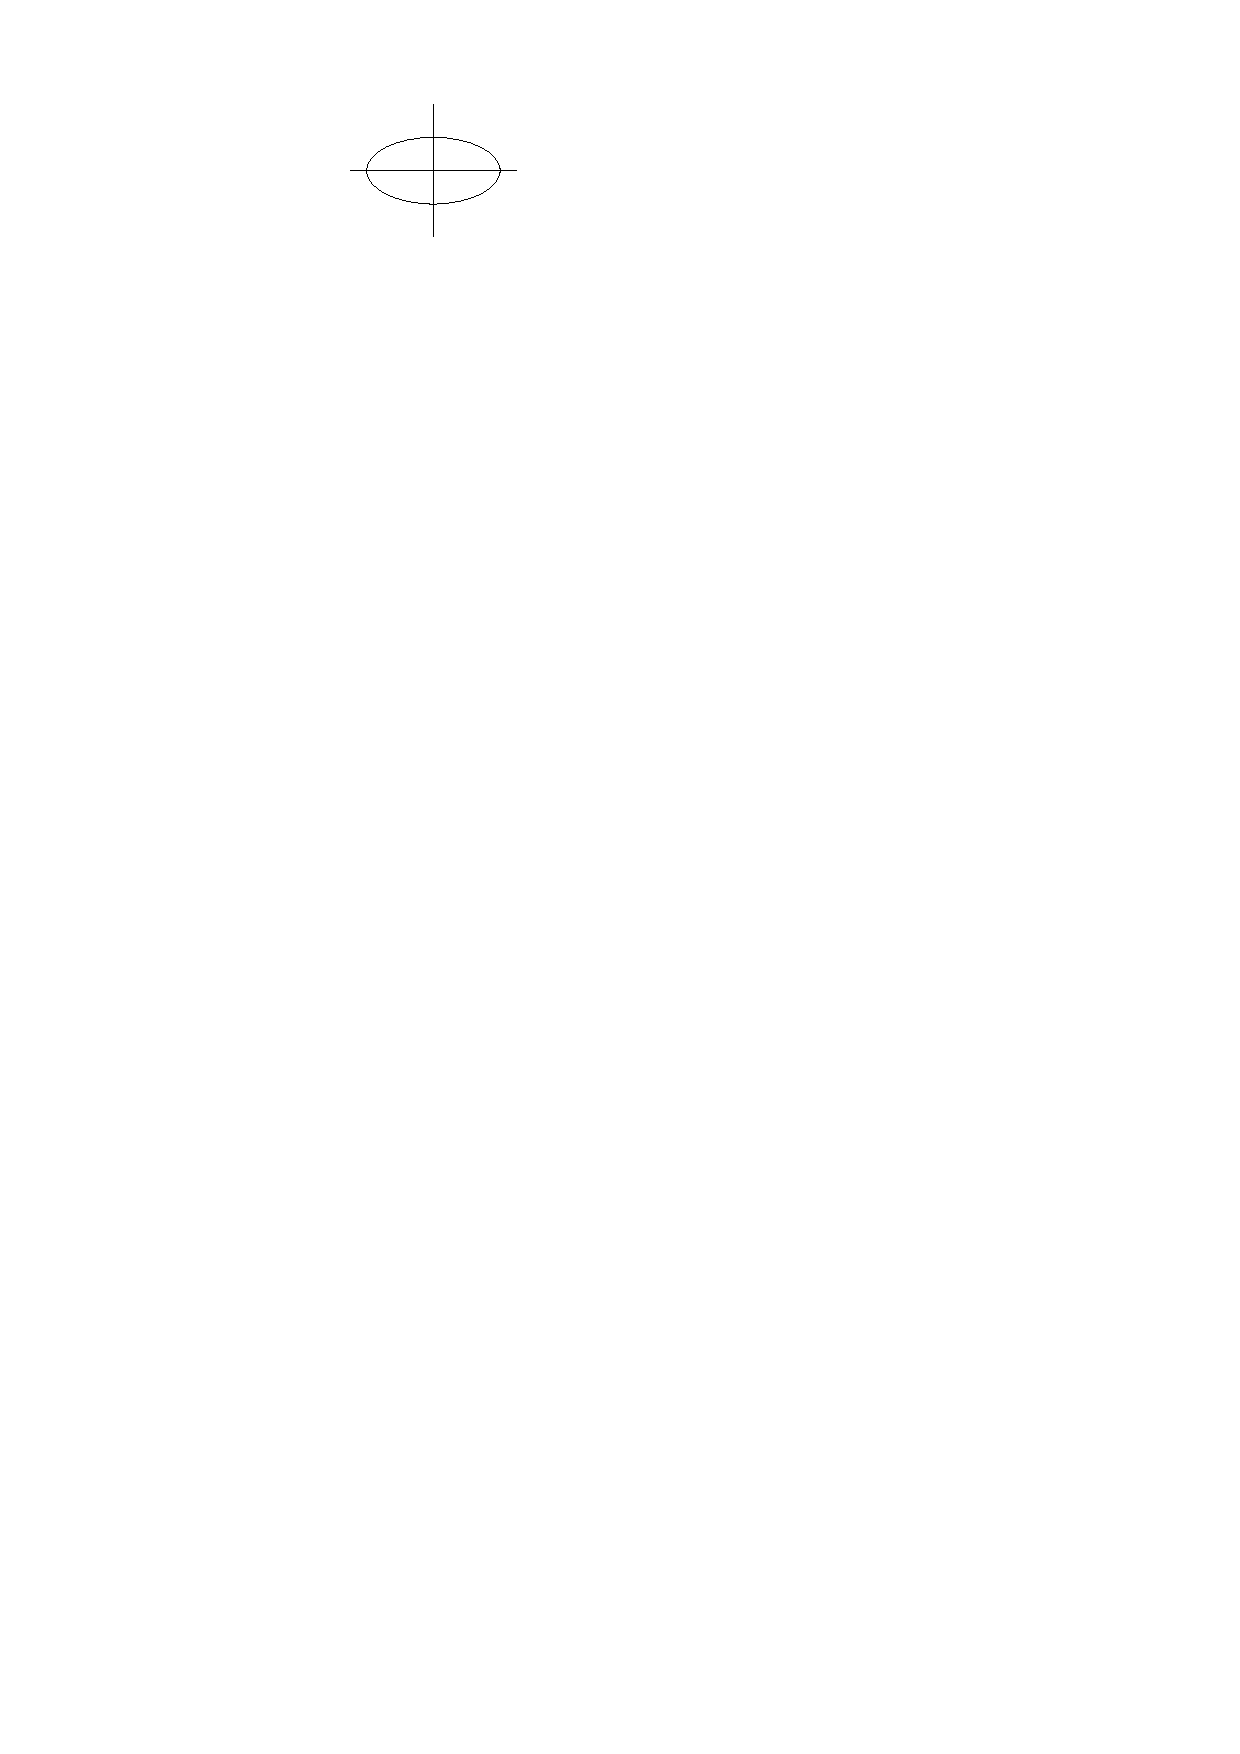
\includegraphics{figures/ueb3/aufgabe5a}
		\caption{Eine Ellipse.}
		\label{fig:ueb3_aufgabe5a}
	\end{figure}

	\item[b, i)] $\vec{r}(t) = (a \cos(\omega t), a \sin(\omega t), c t)$, oder getrennt: $x(t) = a \cos(\omega t)$, $y(t) = a \sin(\omega t)$ und $z(t) = ct$.
	 
	Das ist ein Kreis mit einem linearen "`displacement"' in der $z$-Achse; also eine Art Schraube.
	
	\item[b, ii)] Wir suchen $\Delta z = z(t_2) - z(t_1)$, wobei $x(t_1) = x(t_2)$ und $y(t_1) - y(t_2)$. Man nennt $\Delta z$ auch "`helicoid step"'.
	
	Einsetzen: $x(t_1) = \cos(\omega t_1)$, $x(t_2) = \cos(\omega t_2)$; also $x(t_1) = x(t_2)$ genau dann, wenn $\omega t_1 = \omega t_2 + 2 \pi n$ mit $n \in \mathbb{N}$. Also erfüllt für $\Delta t = \frac{2 \pi}{\omega}$ und Vielfache davon. Damit: $\Delta z = c (t_2 - t_1) = c \Delta t = \frac{2 \pi c}{\omega}$. $\frac{2 \pi}{\omega} =: T$ ist die Periode.
	
	\item[c)] Rechne 
	\begin{align*}
		\vec{v}(t) &= \msimplediff{\vec{r}}{t} = (-r \omega \sin(\omega t), r \omega \cos(\omega t), 0) \\
		\vec{a}(t) &= \msimplediff{\vec{v}}{t} = (-r \omega^2 \cos(\omega t), -r \omega^2 \sin(\omega t), 0) = -\omega^2 \vec{r}(t)
		\text{.}
	\end{align*}
	Siehe Abbildung \ref{fig:ueb3_aufgabe5c} für die Visualisierung der drei Vektoren.
	
	\begin{figure}[h]
		\centering
		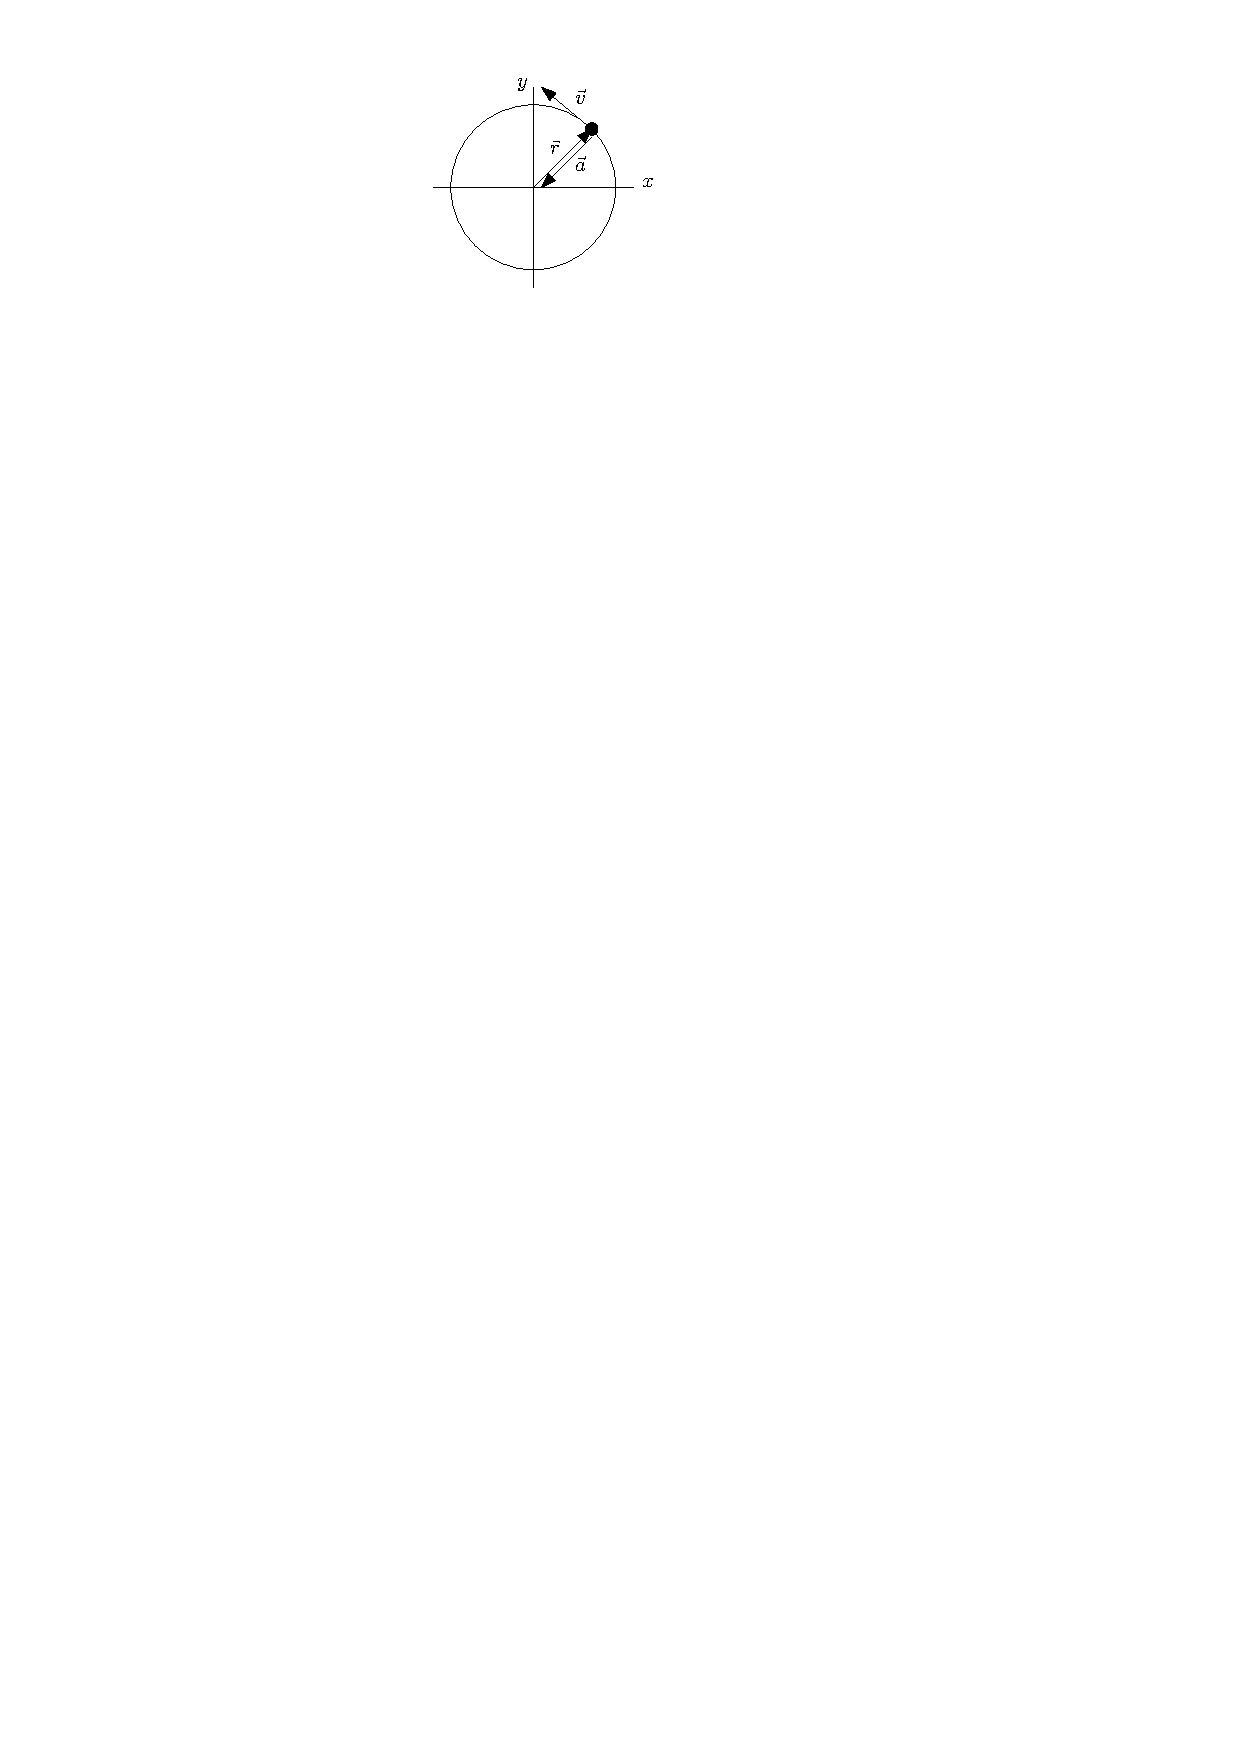
\includegraphics{figures/ueb3/aufgabe5c}
		\caption{Vektore $\vec{r}$, $\vec{v}$ und $\vec{a}$ bei Aufgabe 5c.}
		\label{fig:ueb3_aufgabe5c}
	\end{figure}
	
	Für die Kreisbahn muss nun gelten: $-G \frac{M_e m_s}{r^3} \vec{r} \overset{!}{=} -m_s \omega^2 \vec{r}$. Dass das $m_s$ auf beiden Seiten gleich ist, ist alles andere als trivial und führt auf Einstein zurück; aktuell ist uns das aber egal.
	
	Mit Kürzen erhalten wir
	\[
		-G \frac{M_e}{r^3} \overset{!}{=} -\omega^2 \quad \Rightarrow \quad \omega = \sqrt{ \frac{G M_e}{r} } \frac{1}{r}
		\text{.}
	\]
	
	Beobachtung: $T^2 \approx r^3$; das ist Kepler's Dritte Gesetz.
\end{description}

\section*{Aufgabe 6}

Siehe Abbildung \ref{fig:ueb3_aufgabe6} für eine Skizze. Es gilt $\vec{a} = \msimplediff{\vec{v}}{t}$, also $\mathrm{d} \vec{v} = \vec{a} \mathrm{d} t$. Das integrieren wir:
	\begin{align*}
		& \int_{\vec{v}_0}^{\vec{v}} \mathrm{d} \vec{v}' = \int_{t = 0}^{t} \vec{a} \mathrm{d} t' \\
		\Rightarrow &~ \vec{v} - \vec{v}_0 = (0, 0, -gt) \\
		\Rightarrow &~ \vec{v} = \vec{v}_0 + (0, 0, -gt) = (v \cos(\alpha), 0, v \sin(\alpha) - gt)
		\text{.}
	\end{align*}
	
	Das gleiche Spiel nochmal:
	\[
		\vec{r} = \msimplediff{\vec{v}}{t} 
		\quad \Rightarrow \quad \int_{\vec{r_0}}^{\vec{r}} \mathrm{d} \vec{r}' = \int_{t = 0}^t \vec{v} \mathrm{d} t'
		\quad \Rightarrow \quad \vec{r}(t) - \vec{r}_0 = (v \cos(\alpha t), 0, v \sin(\alpha t) - \frac{1}{2} g t^2)
	\]
	
	Oder getrennt geschrieben: $x(t) = v \cos(\alpha t)$, $y(t) = 0$ und $z(t) = v \sin(\alpha t) - \frac{1}{2} g t^2$. Beobachtung: $z(t)$ wird an zwei Punkten $0$: für $t = 0$ und für $t = \frac{2 v \sin(\alpha)}{g}$.
	
	\begin{figure}[h]
		\centering
		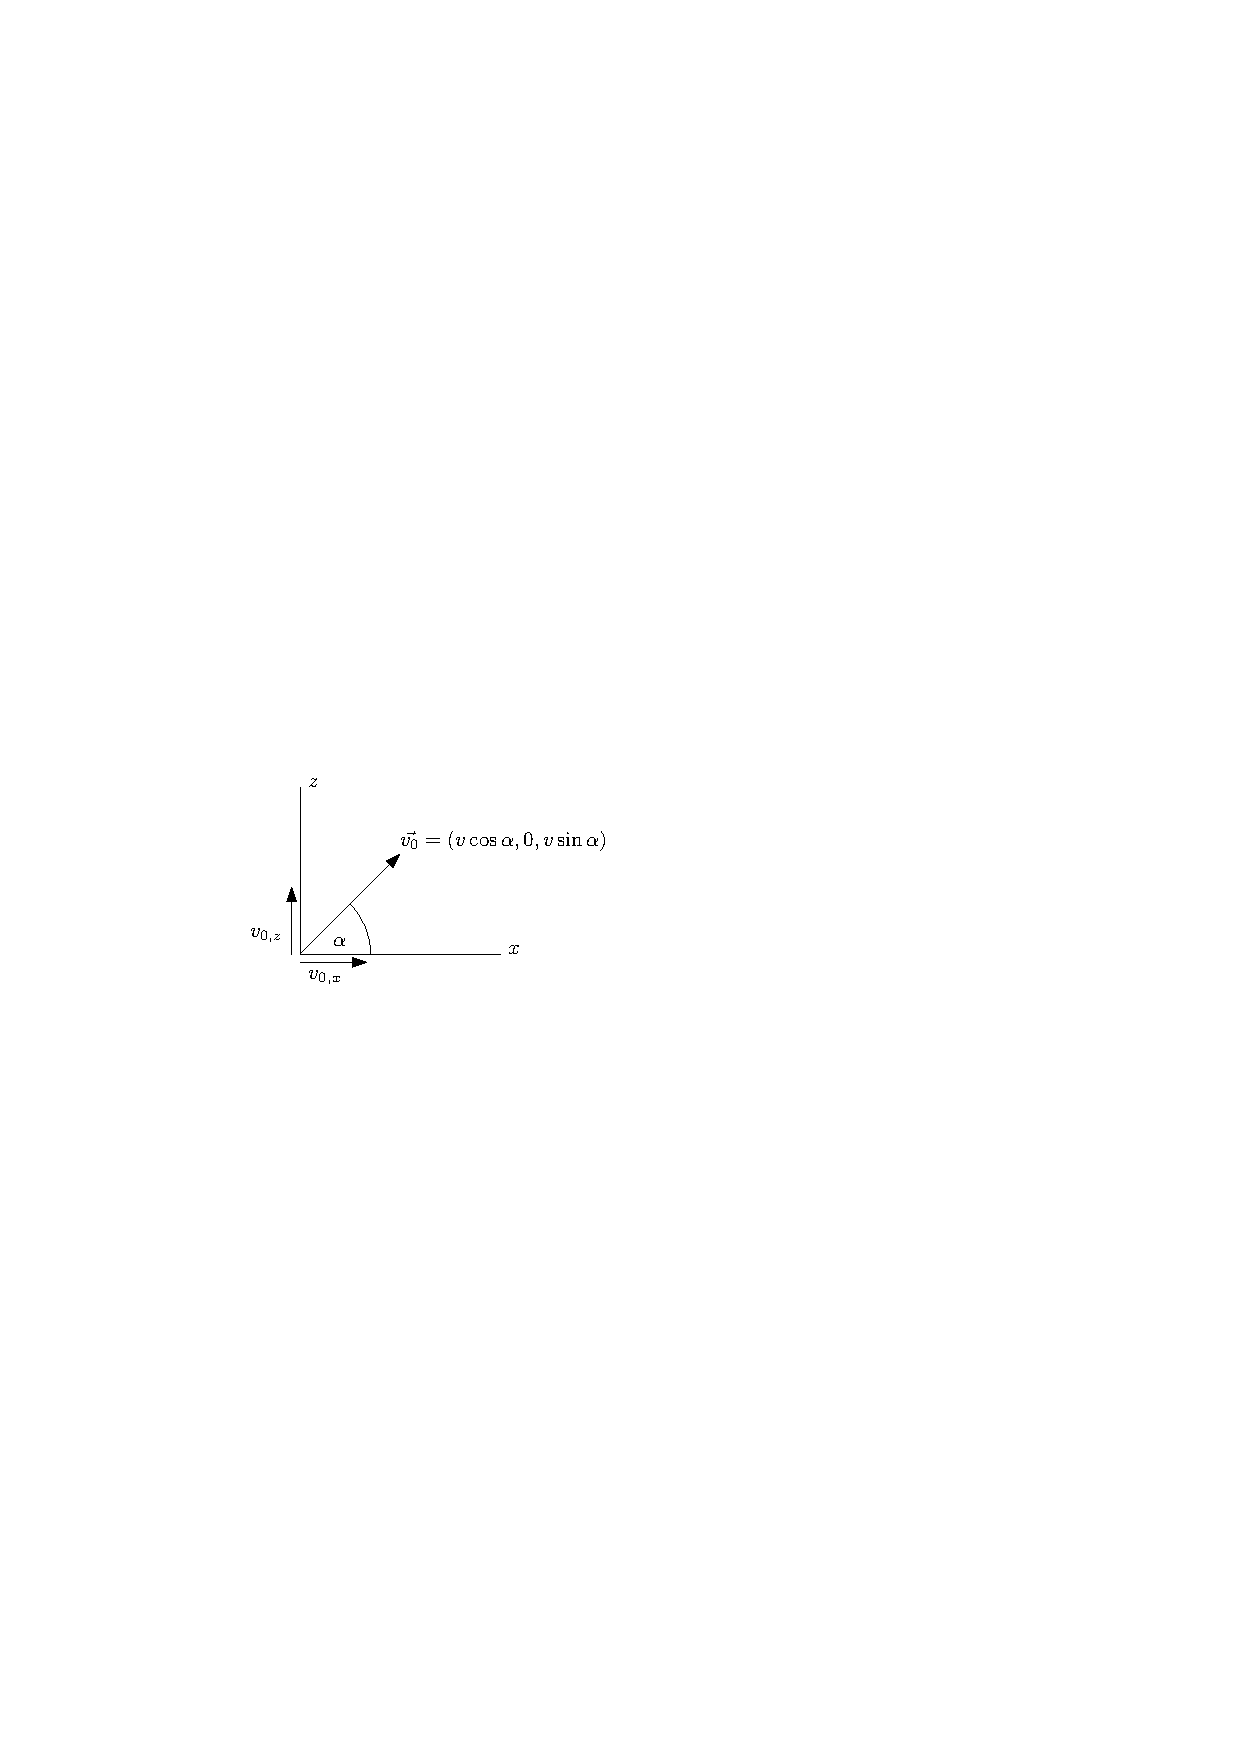
\includegraphics{figures/ueb3/aufgabe6}
		\caption{Eingangssituation in Aufgabe 6.}
		\label{fig:ueb3_aufgabe6}
	\end{figure}
	
	Aus der $x$-Gleichungen erhalten wir $t = \frac{x}{v \cos(\alpha)}$. Also $z(x) = x \tan(\alpha) - \frac{gx^2}{2 v^2 \cos^2(\alpha)}$. Das ist eine Parabel. Die Nullstellen von $z(x)$ sind $x = 0$ und $x = \frac{2 v^2 \sin(\alpha) \cos(\alpha)}{g} = v \cos(\alpha) \underbrace{\frac{2 v \sin(\alpha)}{g}}_{\text{Nullstelle von $z(t)$}}$.
	
	Für welches $\alpha'$ wird ist die Wurfweite maximal? Maximiere $x_{\text{reach}}(\alpha)$. Es gilt
	\[
		\msimplediff{x_{\text{reach}}(\alpha)}{\alpha} = \frac{2v^2}{g} (\cos^2(\alpha) \sin^2(\alpha)) = \frac{2 v^2}{g} \cos(2 \alpha)
		\text{.}
	\]
	Eine Nullstelle $\alpha'$ davon erfüllt $\cos(2 \alpha') = 0$, also $2 \alpha' = \frac{\pi}{2}$ und damit $\alpha' = \frac{\pi}{4}$.

\section*{Aufgabe 7}

Für eine Skizze siehe Abbildung \ref{fig:ueb3_aufgabe7}.

\begin{figure}[h]
	\centering
	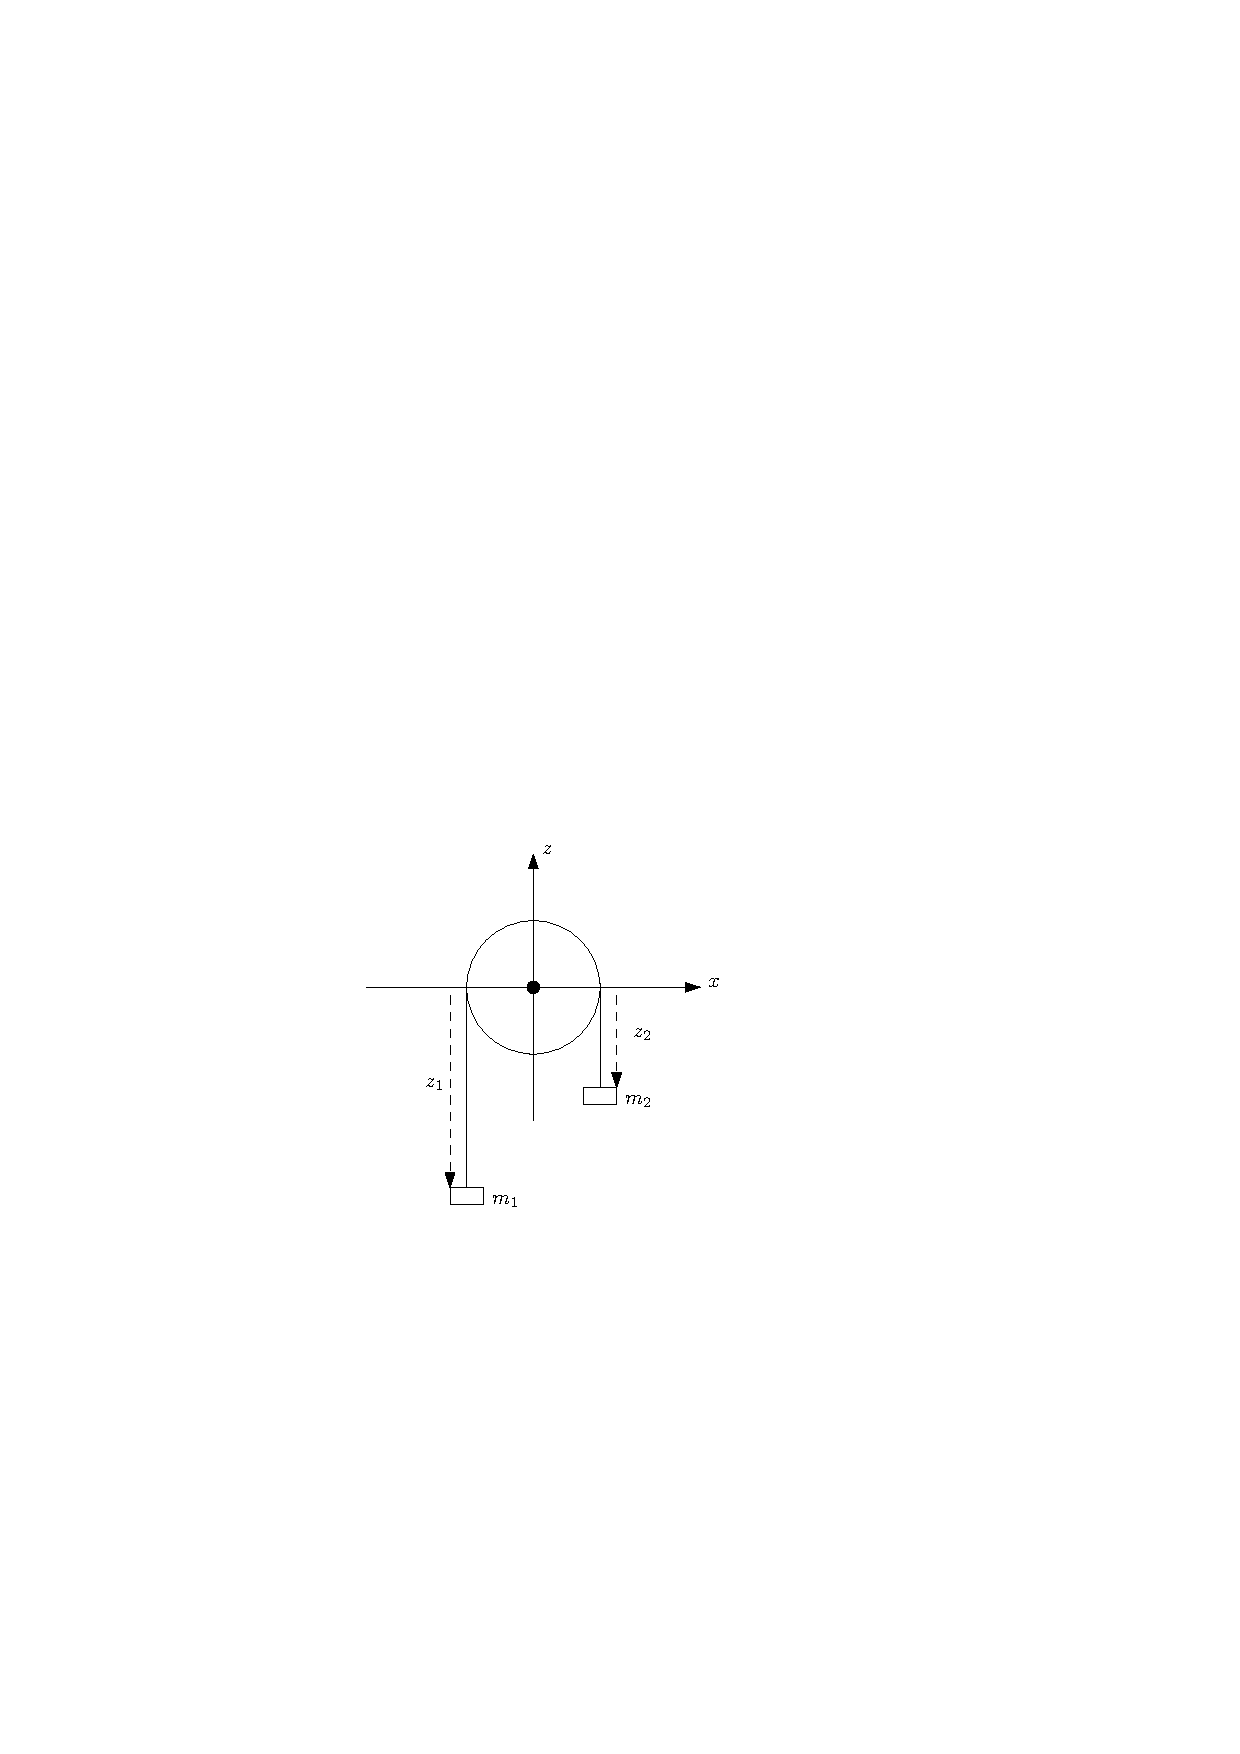
\includegraphics{figures/ueb3/aufgabe7}
	\caption{Die Massen $m_1$ und $m_2$ können sich nur vertikal bewegen.}
	\label{fig:ueb3_aufgabe7}
\end{figure}

Die generalisierten Koordinaten(?,\footnote{nur $(z_1, \dot(z)_1)$ sind generalisierte Koordinaten?}) sind $(z_1, z_2, \dot{z}_1, \dot{z}_2)$ und die Constraints sind Maximale Länge des Fadens, $l = \mabs{z_1} + \mabs{z_2} = -z_1 - z_2$.

Nun die Lagrange-Funktion aufstellen (beachte: $g < 0$, $z_2 = -z_1 - l$, $\dot{z}_2 = \dot{z}_1$): 
\begin{align*}
	L(z_1, z_2, \dot{z}_1, \dot{z}_2) 
	&= T - V = \sum_i T_i - V_i \\
	&= \frac{1}{2} m_1 \vec{z}_1^2 + \frac{1}{2} m_2 \dot{z}_2^2 + m_1 z_1 g + m_2 z_2 g \\
	&= \frac{1}{2} (m_1 + m_2) \dot{z}_1^2 + (m_1 - m_2) g z_1 - m_2 g l
	\text{.}
\end{align*}
Durch das Constraint konnten wir die Lagrange-Funktion also mit nur $(z_1, \dot{z}_1)$ statt $(z_1, z_2, \dot{z}_1, \dot{z}_2)$ ausdrücken.

Anders ausgedrückt: 2 Teilchen, die sich in 1D bewegen, haben zwei Grad Freiheit; das führt auf $4$ Koordinaten. Da wir aber ein Constraint haben, gibt es nur noch ein Grad Freiheit, für das wir nur noch ein Paar Koordinaten brauchen.

Nun muss gelten $\msimplediff{}{t} \frac{\partial L}{\partial \dot{z}_1} = \frac{\partial L}{\partial z_1}$, wobei
\begin{align*}
	\frac{\partial L}{\partial z_1} &= (m_1 - m_2) g, \\
	\msimplediff{}{t} \frac{\partial L}{\partial \dot{z}_1} &= (m_1 + m_2) \ddot{z}_1 
	\text{.}
\end{align*}
Also $(m_1 + m_2) \ddot{z}_1 = (m_1 - m_2) g$ und damit \fbox{$\ddot{z}_1 = g \frac{m_1 - m_2}{m_1 + m_2}$}.

